\chapter*{315 jours, 9100km, 7 pays\markboth{315 jours, 9100km, 7 pays}{}}
\section*{15 janvier 2016}
\subsection*{Chili – 1090km} 
 Pays magnifique pour les paysages et la nature (Patagonie et Atacama). Beaucoup d'autres voyageurs à vélo, bon climat en février/mars : idéal pour démarrer le voyage ! 
\begin{center} 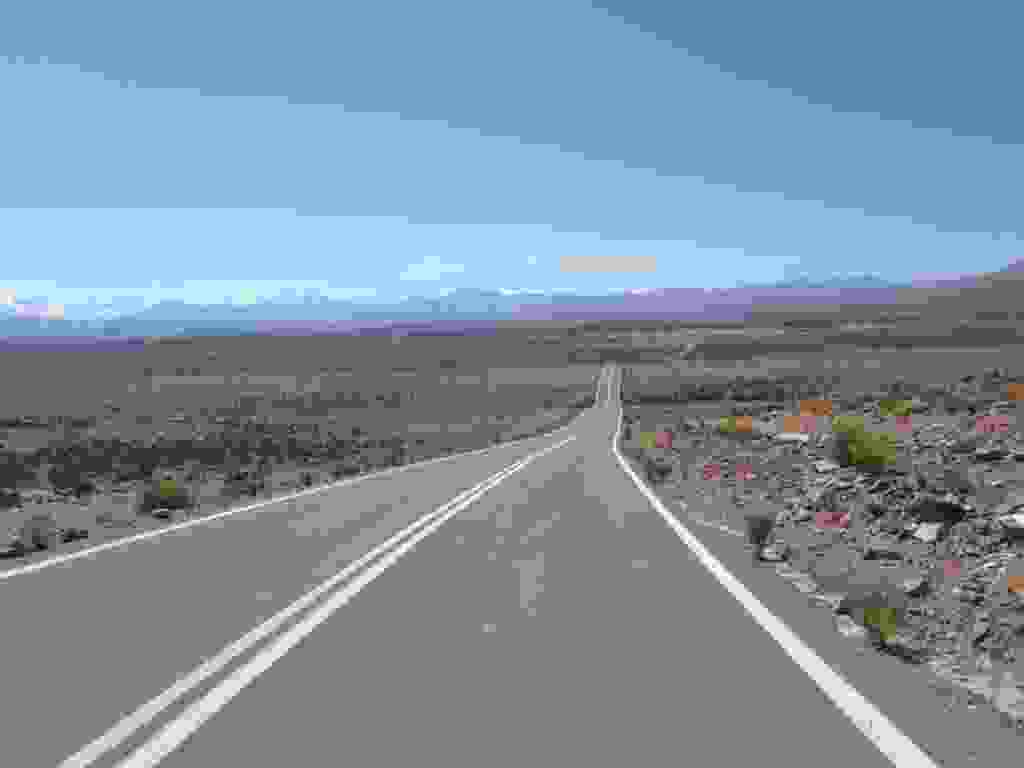
\includegraphics[width=\mywidth]{../wp-content/uploads/2016/01/P3152810-1024x768.jpg} \end{center}
\vspace{-\topsep}
\pagebreak

  \subsection*{Bolivie – 1220km}
 Les 10 jours entre 4000m et 5000m sur les pistes du Sud Lipez restent les plus durs du voyage, heureusement que j'ai rencontré Lucie et Frédéric pour faire cette route bien isolée à plusieurs.

 Le reste était joli mais j'ai moins apprécié à cause des chiens aggressifs et de l'accueil moins chaleureux des locaux dans les campagnes.

 Bon moment à la Casa de Cisclistas de La Paz et avec l'ascension du Huayna Potosi, mon premier 6000m ! 
\begin{center} 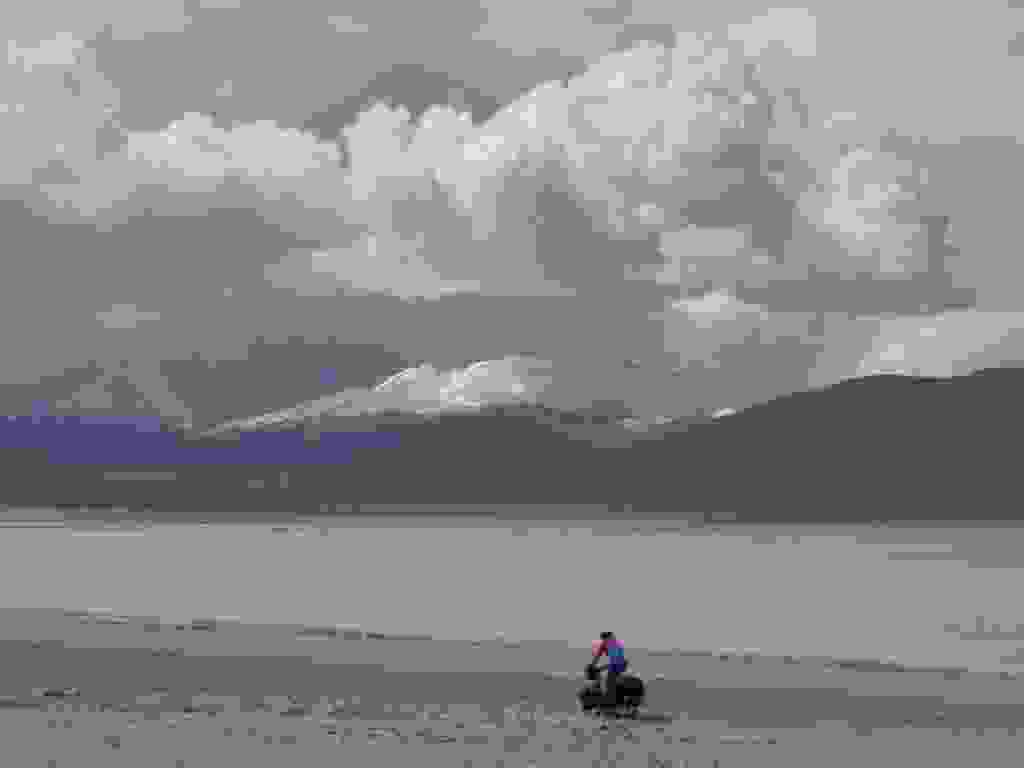
\includegraphics[width=\mywidth]{../wp-content/uploads/2016/01/P1080113-1024x768.jpg} \end{center}
\vspace{-\topsep}
\pagebreak
 
 \subsection*{Pérou – 810km} 
 Accueil très chaleureux, encore beaucoup de cyclistes croisés.

 Les vestiges incas et le cadre naturel autour de Cusco étaient extraordinaires. 

 En général je n'ai pas trop apprécié les tours organisés que j'ai fait, pourtant le trek de 5 jours vers le Macchu Pichu était excellent avec un groupe et un guide super. 
\begin{center} 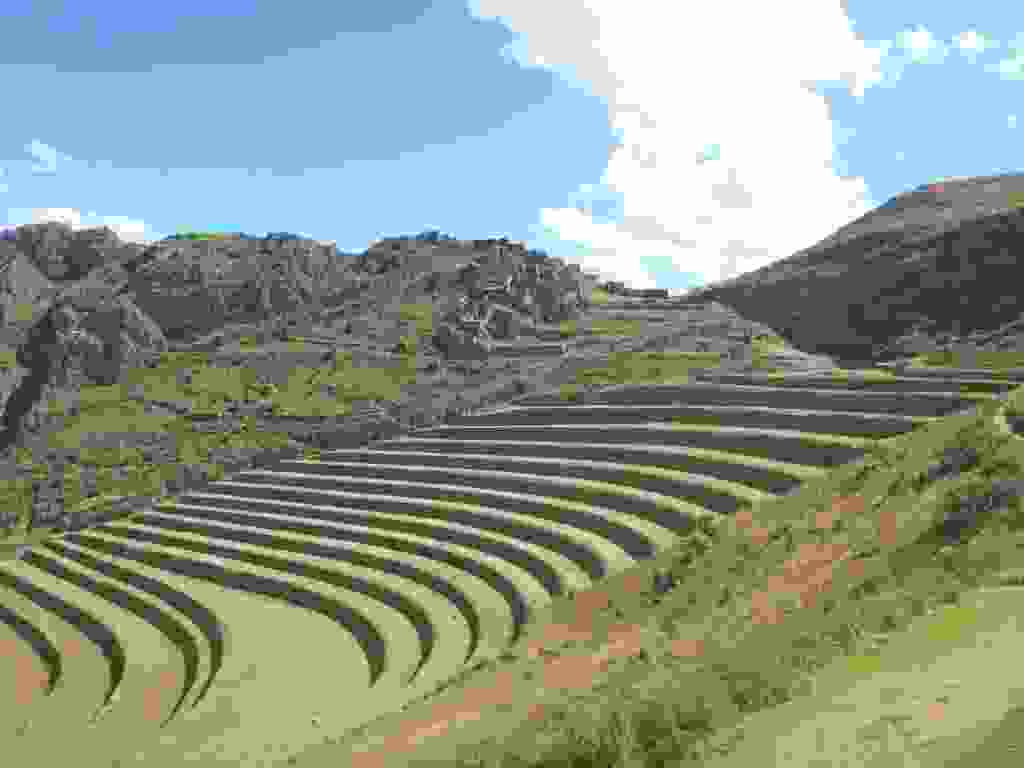
\includegraphics[width=\mywidth]{../wp-content/uploads/2016/01/P5214268-1024x768.jpg} \end{center}
 \vspace{-\topsep}
 \pagebreak
 
 \subsection*{\'Equateur – 480km}
 Un peu déçu par la traversée du pays par la Sierra, peu de rencontres et temps très moyen. Mais aussi un très bon accueil dans des familles près de Quito et une belle journée dans la jungle. 
\begin{center} 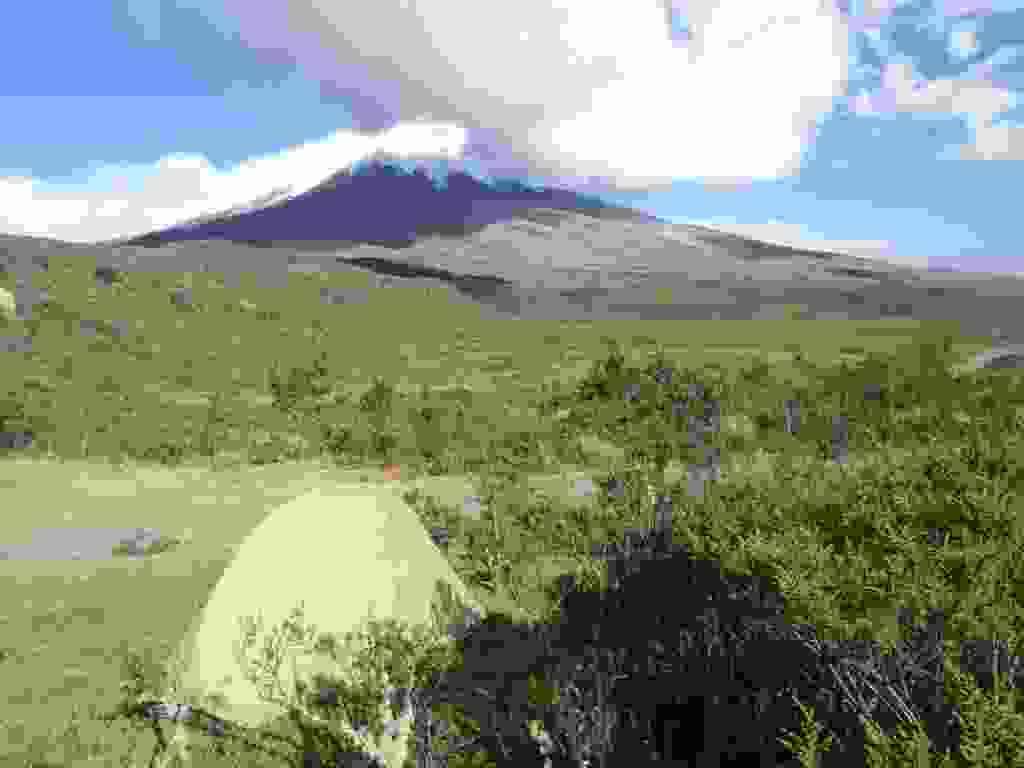
\includegraphics[width=\mywidth]{../wp-content/uploads/2016/01/P6255104-1024x768.jpg} \end{center}
\vspace{-\topsep}
\pagebreak
 
 \subsection*{Japon – 1300km}
 Habitants extraordinaires : toujours courtois et respectueux, dommage que la barrière de la langue empêche souvent d'aller plus loin qu'un premier contact. 

 C'est le pays le plus sûr du monde : il m'a semblé impossible de me faire voler mes affaires et je pouvais poser la tente n'importe où. 

 L'été était très chaud au Japon, même dans les montagnes je n'ai jamais autant transpiré ! 
\begin{center} 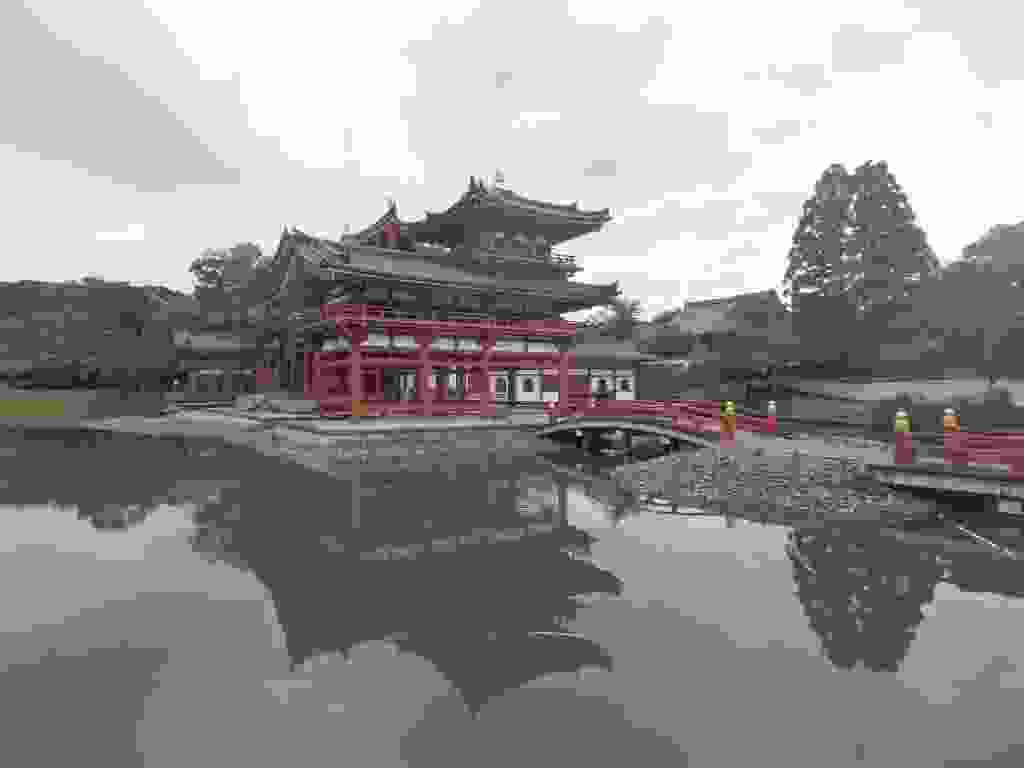
\includegraphics[width=\mywidth]{../wp-content/uploads/2016/01/P8206351-1024x768.jpg} \end{center}
\vspace{-\topsep}
\pagebreak
 
 \subsection*{Chine – 2630km}
 Malgré la communication difficile et la météo très pluvieuse, je me suis très bien senti en Chine. Beaucoup (trop ?) de km et de dénivellé, parfois une dizaine de jours sans croiser d'étrangers, des situations incroyables dans les villages seul au milieu de plein de chinois curieux ! 

 Très bonne cuisine qui ressemblait très peu aux menus des restaurants chinois en France.
\begin{center} 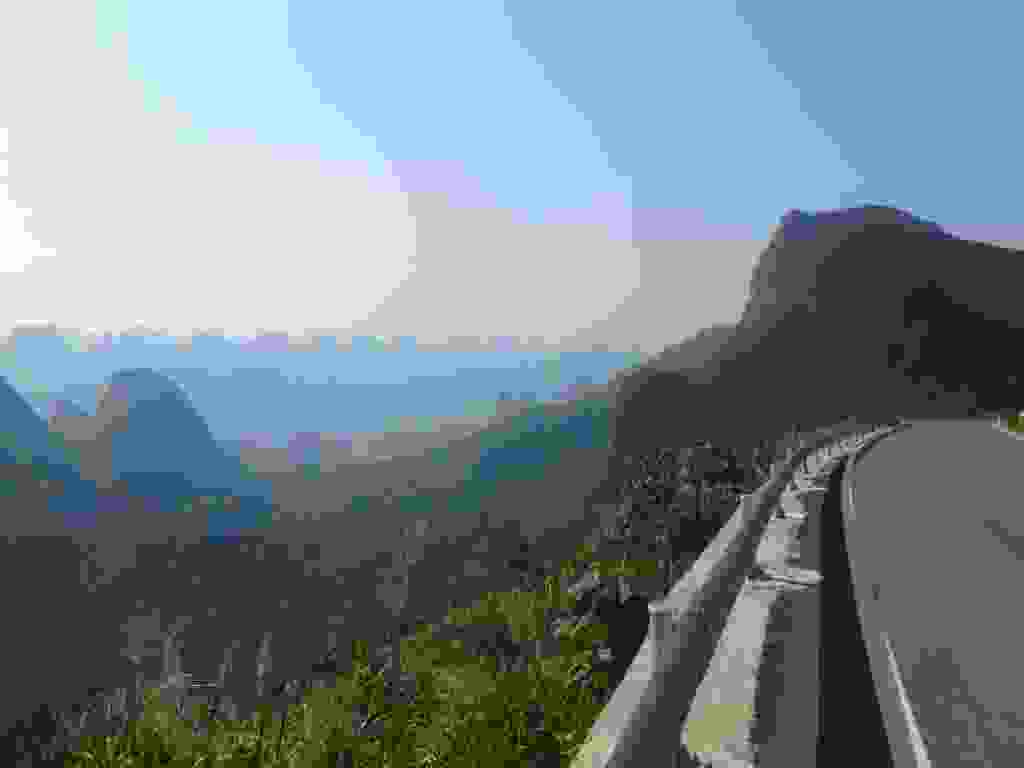
\includegraphics[width=\mywidth]{../wp-content/uploads/2016/01/PA170258-1024x768.jpg} \end{center}
\vspace{-\topsep}
\pagebreak
 
 \subsection*{Inde – 1570km}
 Itinéraire surtout plat mais impossible de s'ennuyer sur la route : toujours des gens pour me saluer ou discuter.

 Bruit, pollution de l'air, déchets partout, la plupart des indiens n'ont aucune conscience du respect de la nature. Malgré cela ils sont sympathiques et ne se plaignent pas. 

 J'ai été quasiment végétarien en Inde, à la fois pour éviter d'être malade et parce que la majorité des restaurants le sont.
\begin{center} 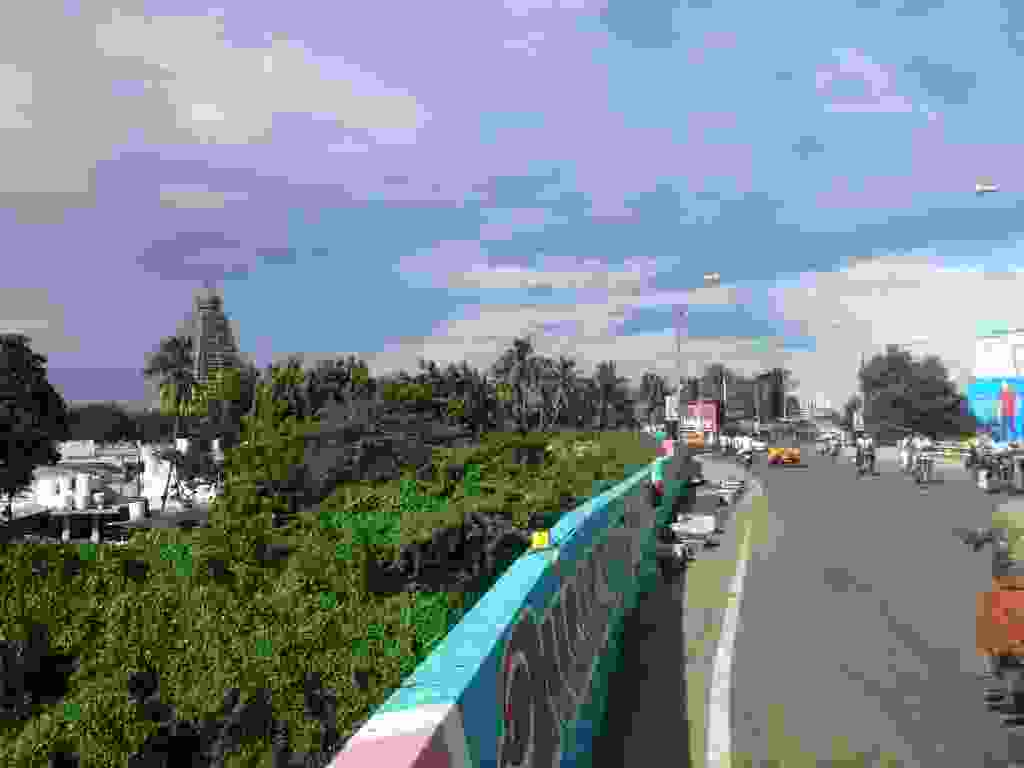
\includegraphics[width=\mywidth]{../wp-content/uploads/2016/01/PB200868-1024x768.jpg} \end{center}
 
 \subsection*{Bilan santé}
 Aucune visite au médecin, seulement 2 touristas en Bolivie et en Inde.

 Une seule petite chute de vélo en Equateur mais pas de blessure.

 \subsection*{Bilan sécurité}
 Pas d'aggression, pas de vol. Seulement le sac à dos \og récupéré \fg\ par quelqu'un en Chine alors qu'il était tombé du porte-bagages. Tous les pays traversés, surtout en Asie sont plus sûrs que la France pour les vols de vélos. 

 Quelques tentatives d'arnaques à Lima, à Shanghai, en Inde dont je me suis tiré sans problème et bien sûr beaucoup d'endroits où j'ai payé le prix «touriste» ou parfois plus, normal !

 \subsection*{Bilan matériel}
 Quelques problèmes mécaniques au début sur des pièces d'origine du VTT d'occasion.

 Seulement 3 crevaisons au total, pas de changement de pneus : les Schwalbe Marathon étaient parfaits. 

 Sacoches Ortlieb excellentes, bien étanches : elles reviennent en très bon état à part celle de la nourriture qui s'est faite manger par des animaux en Inde !

 \subsection*{Bilan personnel} 

 Le plus difficile aura été la décision de partir, beaucoup de doutes avant le départ : Comment se débrouiller seul, surtout dans les endroits dangereux ou reculés ? Les rencontres vont-elles se faire facilement ? Le moral va t'il rester bon ?

 En fait dès les premiers jours, le rythme du voyage est là : chaque jour de nouveaux endroits à découvrir, des rencontres qui arrivent naturellement, des difficultés qui se résolvent facilement et qui entraînent parfois des moments encore meilleurs que s'il ne s'était rien passé.

 Bien sûr quelques moments de solitude ou lassitude qui n'ont jamais durés longtemps. En même temps le voyage à vélo et surtout les moments en bivouac laissent le temps de se poser, de lire, de réfléchir.

 Dans tous les pays, j'ai été accueilli par des habitants de façon spontanée ou grâce aux réseaux d'hospitalité (Warmshowers et Couchsurfing). Partout des gens disponibles pour partager leur temps, offrir à manger parfois en refusant que je débourse le moindre centime.

 Sortir de sa vie quotidienne (au moins temporairement) est possible surtout en France où on a la chance d'avoir le système du congé sabbatique. Pas besoin d'attendre la retraite pour tenter ce qui nous trotte dans la tête...